\documentclass[a4paper, 12pt]{article}
\usepackage[russian]{babel} % Поддержка русского языка
\usepackage{amsmath} % Подключаем пакет для работы с математикой
\usepackage{graphicx} % Подключаем пакет для работы с изображениями
\usepackage{geometry} % Для настройки полей страницы
\geometry{top=2cm, bottom=2cm, left=2cm, right=2cm} % Устанавливаем поля

\begin{document}

\begin{titlepage}
    \centering
    \vspace*{2cm}
    
    {\Large Санкт-Петербургский Политехнический университет Петра Великого \par}
    \vspace{1.5cm}
    
    {\huge Отчет по лабораторной работе №4 \par}
    {\huge по дисциплине "Интервальный анализ" \par}
    \vspace{2cm}
    
    {\Large Линейная регрессия\par}
    \vfill
    
    \begin{flushright}
Выполнил студент:
Асанов Дамир \\   
группа:
5030102/10201\\
Проверил:
доцент
Баженов Александр Николаевич
\end{flushright}
\end{titlepage}



\newpage % Начать новую страницу для содержания
\tableofcontents


\newpage
\section{Постановка задачи}

Дан измеритель, на вход которого поступает калибровочный сигнал - набор постоянных напряжений
\begin{center}
    $X = \lbrace x_i \rbrace ^{100}_{i = 1}$
\end{center}
а данные на выходе - набор интервальных данных
\begin{center}
    $Y = \lbrace y _k \rbrace ^{100}_{k = 1}$, rad $y = \frac{1}{2^N}B$, $N = 14$
\end{center} 
Файлы данных хранятся в бинарном формате и считывается в соответствии со следующим преобразованием:
\begin{center}
    $V = \textit{Code}/16384 - 0.5$
\end{center} 

Необходимо оценить значения $\beta _0$ и $\beta _1$ - параметров  линейной регрессии
\begin{center}
    $y = \beta _0 + \beta _1 * x$
\end{center}

Оценки значений $Y$:
\begin{itemize}
    \item внутренняя (in) - интервал между первым и третьим квартилем
    \item внешняя (ex) -  границы бокс-плота
\end{itemize}
\vspace{5mm}
Требуется:
\begin{itemize}
    \item Решить ИСЛАУ (1) для внутренних и внешних оценок $y$
    \item Построить множество решений $\beta _0$, $\beta _1$
    \item Построить коридор совместных зависимостей, используя пример — \\https://github.com/szhilin/octave-interval-examples/
blob/master/SteamGenerator.ipynb
\end{itemize}


\section{Теоретическое обоснование}

\subsection{Бокс-плот Тьюки}
Боксплот (англ. box plot) — график, использующийся в описательной статистике, компактно изображающий одномерное распределение вероятностей. Такой вид диаграммы в удобной форме показывает медиану, нижний и верхний квартили и выбросы. Границами ящика служат первый и третий квартили, линия в середине ящика — медиана. Концы усов - края статистически значимой выборки (без выброса). Длину «усов» определяют разность первого квартиля и полутора межквартальных расстояний и сумма третьего квартиля и полутора межквартальных расстояний. Формула имеет вид\\
$X_1 = Q_1 - \frac{3}{2}(Q_3 - Q_1)$, $X_2 = Q_3 + \frac{3}{2}(Q_3 - Q_1)$
\\где $X_1$ - нижняя граница уса, $X_2$ — верхняя граница уса, $Q_1$ — первый квартиль, $Q_3$ - третий квартиль. Данные, выходящие за границы усов (выбросы), отображаются на графике в виде маленьких кружков. Выбросами считаются величины , такие что:\\
$\left[ \begin{gathered}
x < X_1^T\\
x > X_2^T
\end{gathered} \right.$

\subsection{Интервальная мода}
Пусть имеется интервальная выборка\\
$X = \lbrace x_i \rbrace$
Сформируем массив интервалов z из концов интервалов X.
\\Для каждого интервала $z_i$ подсчитываем число $\mu _i$ интервалов из выборки $X_i$, включающих $z_i$. Максимальные $\mu _i$ = max $\mu$ достигаются для индексного множества K. Тогда можно найти
интервальную моду как мультиинтервал\\
mode X = $\bigcup_{k \in K}{z_k}$

\subsection{Интервальная медиана Крейновича}
Пусть дана выборка X = {$x_i$}. Пусть $\underline{c}$ = {$\underline{x_i}$}, $\overline{c}$ = {$\overline{x_i}$} — конфигурация точек, составленные, соответственно, из левых и правых концов интервалов из X. Медиана Крейновича $med_{K}X$ интервальной выборки X — это интервал\\ $med_K$ = [$med_{\underline{c}}$, $med_{\overline{c}}$].

\subsection{Интервальная медиана Пролубникова}
Зададим отношения порядка на алгебре $\mathbb{R}$. Говорят, что неравенство $a \leq b$ выполняется\\
\begin{enumerate}
    \item в сильном смысле, если $\forall a \in \mathbb{R}$ $ \forall b \in \mathbb{R}$ : $\overline{a} \leq \underline{b}$
    \item в слабом смысле, если $\exists a \in \mathbb{R}$ $ \exists b \in \mathbb{R}$ : $\underline{a} \leq \overline{b}$
    \item в $\forall \exists$-смысле, если $\forall a \in \mathbb{R} $ $ \exists b \in \mathbb{R}$ : $\underline{a} \leq \underline{b}$
    \item в $\exists \forall$-смысле, если $\exists a \in \mathbb{R}$ $\forall b \in \mathbb{R}$ : $\overline{a} \leq \overline{b}$
    \item в центральном смысле, если $\frac{\overline{a} + \underline{a}}{2} \leq \frac{\overline{b} + \underline{b}}{2}$
\end{enumerate}
Для элементов выборки X можно определить линейный порядок, используя любое из пяти
вышеуказанных отношений порядка на $\mathbb{R}$. То есть, если $i \neq j$, то либо $x_i \leq x_j$ , либо $x_i \geq x_j$ для любого из этих отношений порядка.\\
Медиана Пролубникова $med_{P}{X}$ выборки X — это интервал $x_m$, для которого половина интервалов из X лежит слева, а половина — справа.\\
В ситуации, когда имеются два элемента подинтервала $x_m$ и $x_{m + 1}$, расположенных посередине вариационного ряда, $x_m \neq x_{m + 1}$ медиана может быть определена естественным обобщением взятия полусуммы точечных значений, расположенных посередине ряда из точечных значений, в случае интервальной выборки взятие полусуммы интервалов $x_m$ и $x_{m + 1}$:\\
$med_{P}{X} = \frac{x_m + x_{m + 1}}{2}$.

\section{Описание работы}

Лабораторная работа выполнена на языке программирования Python в среде разработки VSCode. В ходе работы были использованы следующие библиотеки: numpy, scipy, intervalpy
и matplotlib. GitHub репозиторий: \texttt{https://github.com/theguydie/interval-analysis}

\subsection{Описание алгоритма}
Каждый из 8 файлов содержит 100 фреймов, каждый из которых включает 1024 массива, состоящих из 8 двухбайтовых значений. В результате обработки этих данных было сформировано 1024 × 8 = 8192 ИСЛАУ, представленных в следующем виде:\\

\[ \begin{pmatrix}
         [$x_1$, $x_1$] & [1,1]\\ 
         $\vdots$ & $\vdots$\\
         [$x_8$, $x_8$] & [1,1]
     \end{pmatrix}
     \times
     \begin{pmatrix}
         $\beta _1$\\ 
         $\beta _0$ 
     \end{pmatrix}
      =
     \begin{pmatrix}
         $\widehat{y_1_i}$\\
         $\vdots$\\
         $\widehat{y_8_i}$
     \end{pmatrix} \]
     \begin{itemize}
        \item j — порядковый номер файла, $j \in \overline{1, 8}$
        \item i — номер пикселя внутри файла, $i \in \overline{1, 8192}$
        \item $x_j$ — вольтаж, определяемый по первой цифре названия файла
        \item $\widehat{y_j_i}$ — оценка значения, соответствующее каждому пикселю, по всем 100 фреймам
        \item $\beta _0$ и $\beta _1$ — искомые параметры линейной регрессии. 
     \end{itemize}
     
Каждая система линейных алгебраических уравнений была решена с использованием метода Дж. Рона [1], реализованном в библиотеке intervalpy. В результате были получены два множества интервалов оценок: $B_0$ = $\lbrace \beta _0 \rbrace ^{8192} _{i = 1}$ и $B_1$ = $\lbrace \beta _1 \rbrace ^{8192} _{i = 1}$ \\

Оценка каждого из параметров
линейной регрессии будем производить следующим образом:

\begin{enumerate}
    \item $\widehat{\beta _0}$ = $med_{K}{B_0}$, $\widehat{\beta _1}$ = $med_{K}{B_1}$
    \item $\widehat{\beta _0}$ = $med_{P}{B_0}$, $\widehat{\beta _1}$ = $med_{P}{B_1}$
    \item $\widehat{\beta _0}$ = mode${B_0}$, $\widehat{\beta _1}$ = mode${B_1}$
\end{enumerate}

Таким образом, конечные значения $\widehat{\beta _0}$ и $\widehat{\beta _1}$ служат наиболее вероятными оценками параметров регрессии, что позволяет более точно анализировать зависимость между переменными в исследуемых данных.

\section{Результаты}
\subsection{Оценки}
В ходе лабораторной работы для внутренней оценки были получены следующие результаты:\\
\begin{itemize}
    \item $\bigcap_{i = 1}^{8192}$, $ \beta _{0, i} = \emptyset$
    \item $\bigcap_{i = 1}^{8192} \beta _{1, i} = \emptyset$
    \item $med_{K}{B_0}$ = [8029.18, 8190.85] и $med_{K}{B_1}$ = [12857.0, 13289.5] для внутренней оценки медианой Крейновича
    \item $med_{P}{B_0}$ = [8023.65, 8195.88] и $med_{P}{B_1}$ = [12879.9, 13280.5] для внутренней оценки медианой Пролубникова
    \item mode${B_0}$ = {[8083.32, 8083.33], [8086.78, 8086.80]} и mode${B_1}$ = [13070.5, 13072.5] для внутренней оценки модой.
\end{itemize}

Для внешней оценки были получены следующие результаты:\\
\begin{itemize}
    \item $\bigcap_{i = 1}^{8192} \beta _{0, i} = \emptyset$
    \item $\bigcap_{i = 1}^{8192} \beta _{1, i} = \emptyset$
    \item $med_{K}{B_0}$ = [7780.52, 8430.21] и $med_{K}{B_1}$ = [12193.0, 13950.3] для внутренней оценки медианой Крейновича
    \item $med_{P}{B_0}$ = [7765.31, 8454.22] и $med_{P}{B_1}$ = [12279.1, 13881.3] для внутренней оценки медианой Пролубникова
    \item mode${B_0}$ = [7927.51, 8224.58] и mode${B_1}$ = [13097.9, 13573.8] для внутренней оценки модой.
\end{itemize}

\subsection{Графики}

\begin{figure}[ht!]
  \centering
\begin{minipage}[b]{0.4\textwidth}
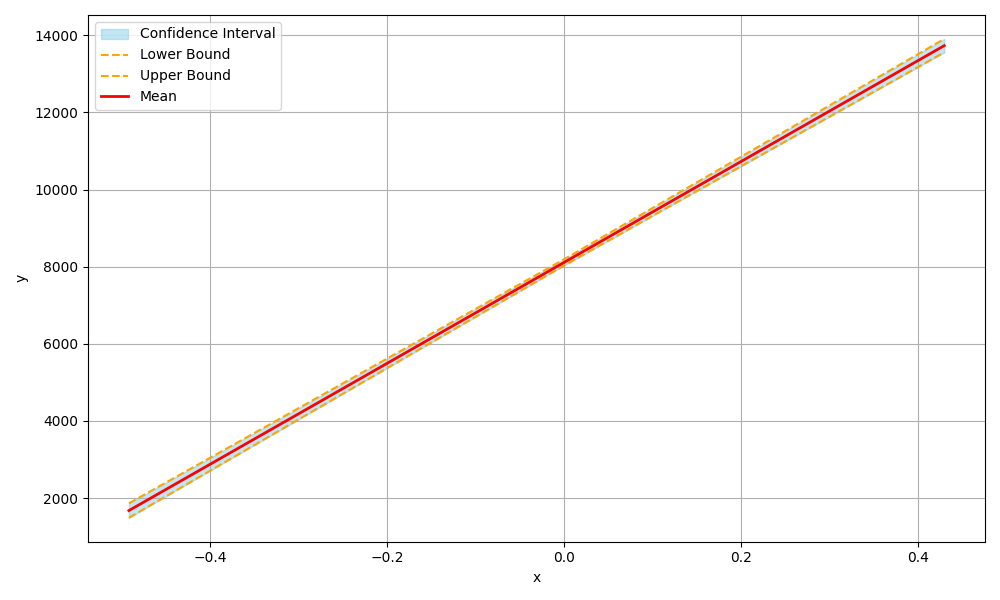
\includegraphics[width=3.0in, height=2.7in] {Медиана Крейновича in.png}
\caption{Коридор совместных зависимостей для внутренней оценки медианой Крейновича} 
\end{minipage}
\hfill
\begin{minipage}[b]{0.4\textwidth}
  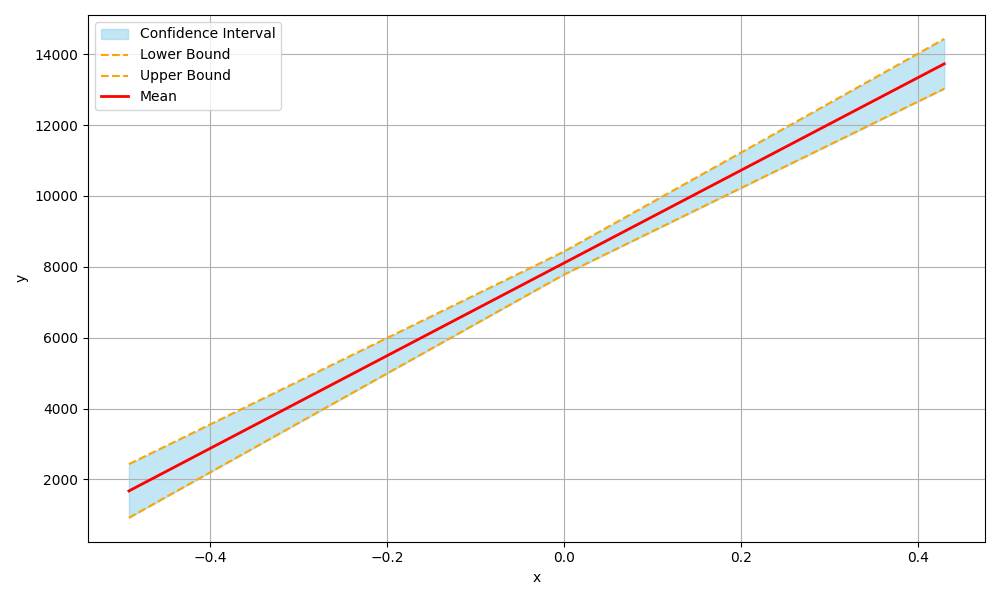
\includegraphics[width=3.0in, height=2.7in]{Медиана Крейновича ext.png}
 \caption{Коридор совместных зависимостей для внешней оценки медианой Крейновича.}
\end{minipage}
\end{figure}

\begin{figure}[ht!]
  \centering
\begin{minipage}[b]{0.4\textwidth}
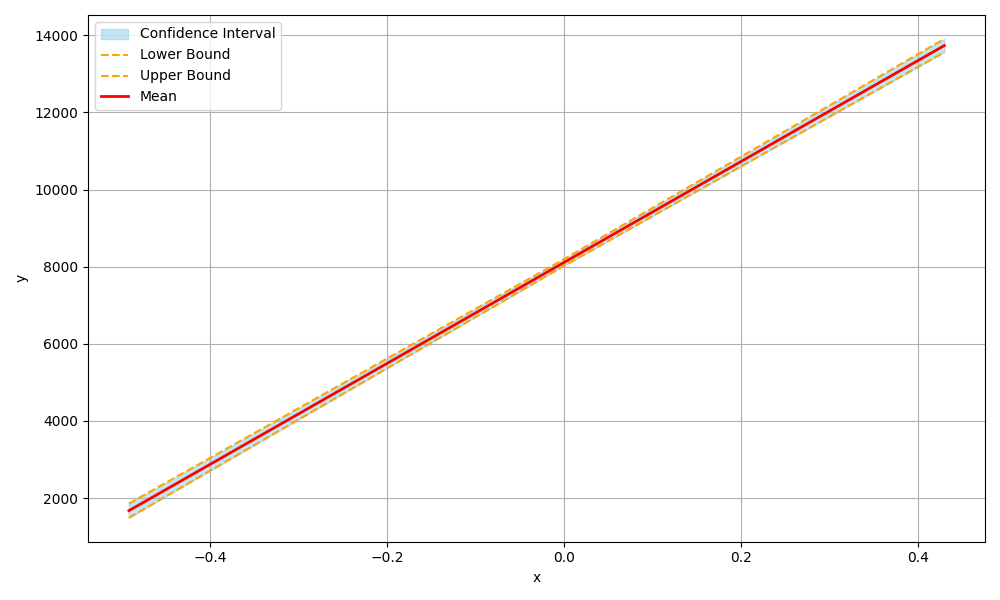
\includegraphics[width=3.0in, height=2.7in] {Медиана Пролубникова in.png}
\caption{Коридор совместных зависимостей для внутренней оценки медианой Пролубникова} 
\end{minipage}
\hfill
\begin{minipage}[b]{0.4\textwidth}
  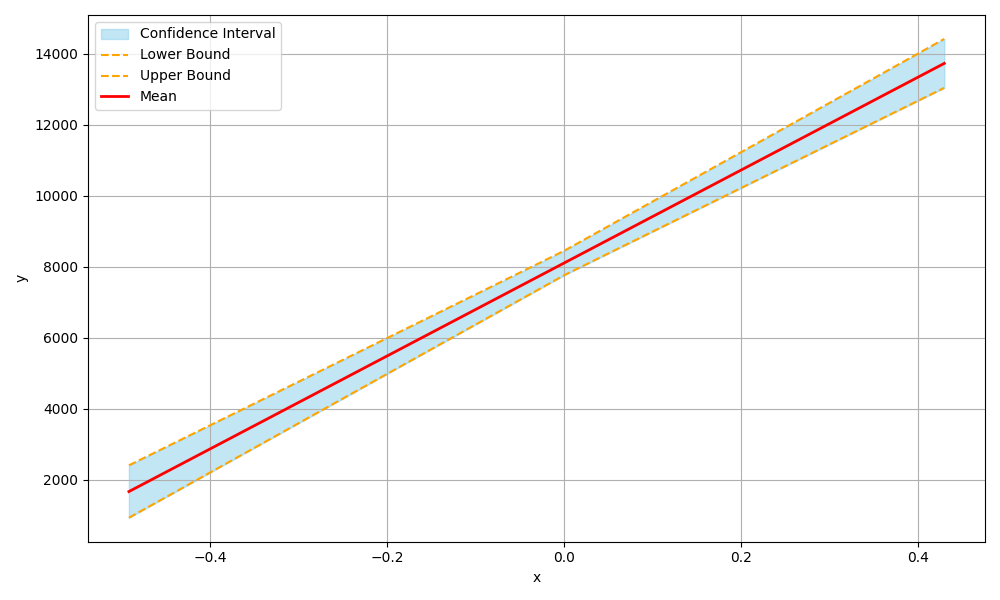
\includegraphics[width=3.0in, height=2.7in]{Медиана Пролубникова ext.png}
 \caption{Коридор совместных зависимостей для внешней оценки медианой Пролубникова}
\end{minipage}
\end{figure}

\begin{figure}[ht!]
  \centering
\begin{minipage}[b]{0.4\textwidth}
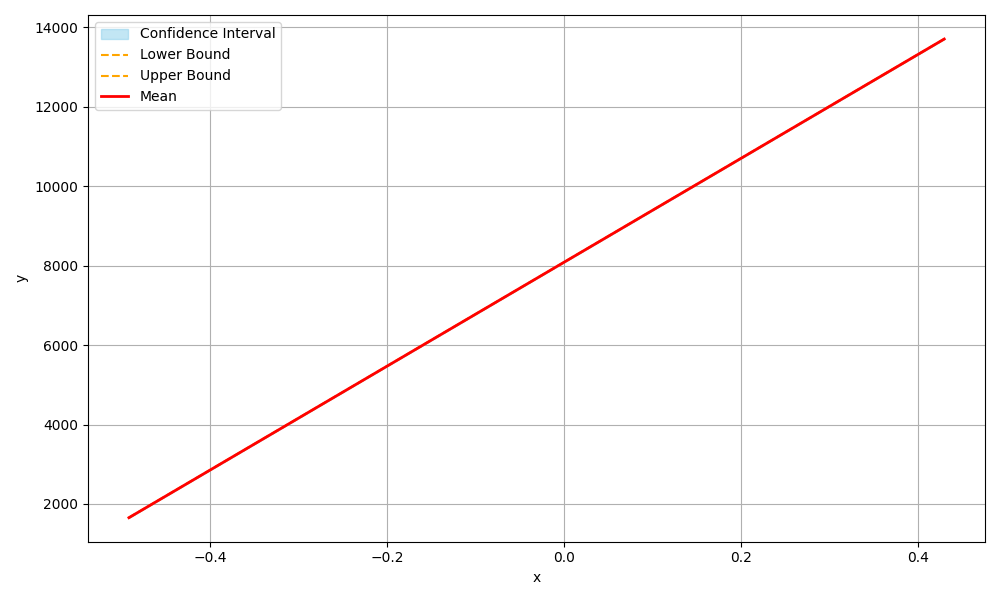
\includegraphics[width=3.0in, height=2.7in] {Мода in.png}
\caption{Коридор совместных зависимостей для внутренней оценки модой} 
\end{minipage}
\hfill
\begin{minipage}[b]{0.4\textwidth}
  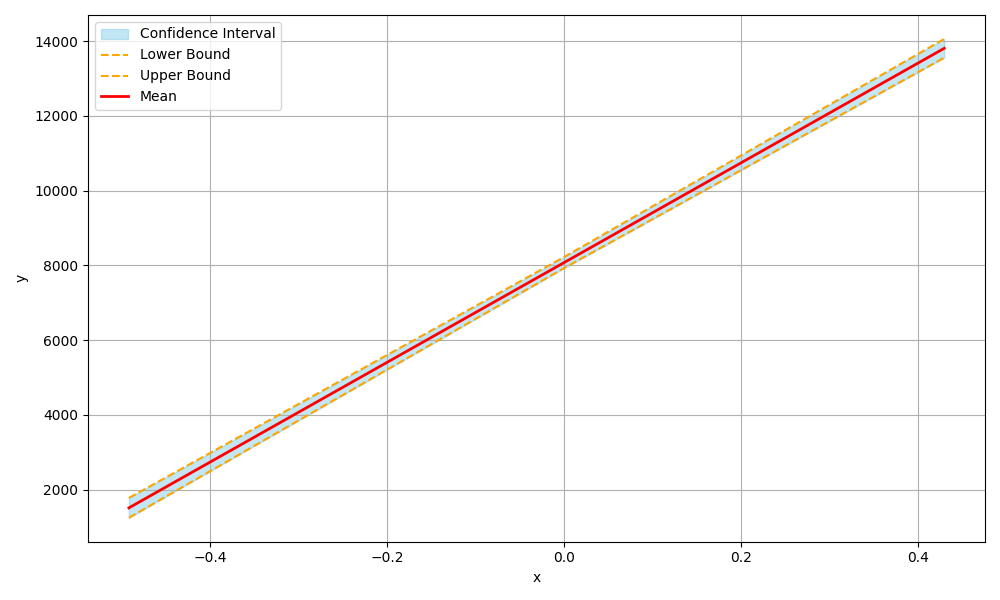
\includegraphics[width=3.0in, height=2.7in]{Мода ext.png}
 \caption{Коридор совместных зависимостей для внешней оценки модой}
\end{minipage}
\end{figure}

\newpage
\section{Заключение}
В процессе выполнения лабораторной работы была разработана методика для оценки параметров линейной регрессии на основе интервальных данных. Основные достижения включают:
\begin{itemize}
    \item Создан алгоритм для вычисления внутренних и внешних оценок параметров линейной
регрессии, что позволяет учитывать неопределённость в исходных данных
    \item Получены интервальные оценки параметров $\beta _0$ и $\beta _1$, которые демонстрируют диапазон
возможных значений параметров регрессии.
    \item Построены коридоры совместных зависимостей, визуализирующие интервальные решения и способствующие анализу устойчивости модели
\end{itemize}
Полученные результаты свидетельствуют о том, что предложенный подход обеспечивает более точное моделирование зависимостей в данных, принимая во внимание возможные вариации
и ошибки. Это особенно актуально в тех областях, где точность измерений может изменяться,
и требуется надежная оценка параметров модели.

\section{Литература}
\begin{enumerate}
    \item A.Н.Баженов. Интервальный анализ. Основы теории и учебные примеры. СПБПУ. 2020.
    \item J. Rohn — «Enclosing solutions of overdetermined systems of linear interval equations», Reliable
Computing 2 (1996), 167-171.
\end{enumerate}

\end{document}
